\documentclass[convert]{standalone}

\usepackage{tikz}
\usepackage{graphicx}
\pagestyle{empty}

% INT_AY20_MP3_L22_Fig04_RHR-forces.tex

\begin{document}
\begin{tikzpicture}[> = latex, scale = 0.50, font = \Huge]

	% Original file
	
	% source: https://commons.wikimedia.org/wiki/File:Right_hand_rule_cross_product.svg
	
	\node at (0, 0) {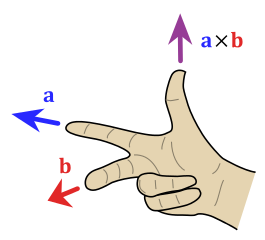
\includegraphics{Right_hand_rule_cross_product.svg.png}};
	
	% Modify file to put vectors for magnetic force RHR
	
	\draw [fill = white, draw = none] (-7, 1) rectangle (-5, 3);
	\node at (-6, 2) {${\vec v}$};
	
	\draw [fill = white, draw = none] (-6, -4) rectangle (-4, -2);
	\node at (-5, -3) {${\vec B}$};
	
	\draw [fill = white, draw = none] (4.5, 5) rectangle (8, 7);
	\node at (6, 6) {${\vec F}_m$};

\end{tikzpicture}
\end{document}